\documentclass{article}
\usepackage{tikz}
\usetikzlibrary{shapes}
\usepackage[utf8]{inputenc}
\begin{document}
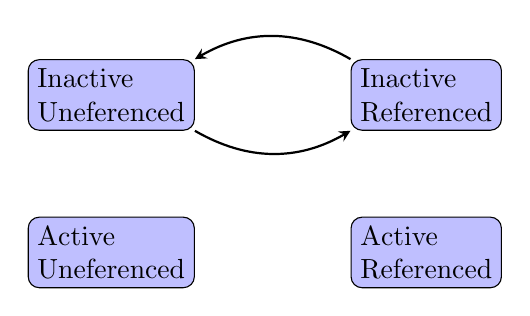
\begin{tikzpicture}
% style des nœuds
\tikzstyle{state}=[rectangle,draw,rounded corners=4pt,fill=blue!25, align=left]
% style des flèches
\tikzstyle{transition}=[->,>=stealth,thick,rounded corners=4pt]
% placement des nœuds
\node[state] (AU) at (0,0) {Active \\ Uneferenced};
\node[state] (IU) at (0,2) {Inactive \\ Uneferenced};
\node[state] (AR) at (4,0) {Active \\ Referenced};
\node[state] (IR) at (4,2) {Inactive \\ Referenced};
% Placement des flèches
\draw[transition] (IU.south east) to [bend right] (IR.south west);
\draw[transition] (IR.north west) to [bend right] (IU.north east);

\end{tikzpicture}
\end{document}